\chapter{The Standard Model and Extensions}\label{chapter:theory}

\section{The Standard Model}\label{section:standard_model}

The Standard Model of particle physics is the collection of \glspl{QFT} that describes the interactions of elementary matter with three of the four%
\footnote{Gravity is noticeably absent, as at the time of writing there is no working quantum theory of gravitation.}
known forces of Nature: the electromagnetic force, the weak nuclear force, and the strong nuclear force.
These theories collectively form a symmetry group%
\footnote{$\mathrm{SU}(n)$ is the special unitary group of degree $n$ which is the Lie group  of $n\times n$ unitary matrices with determinant of $1$.
 As the group is non-Abelian the gauge symmetries that belong to these groups are known as ``non-Abelian gauge symmetires.''}
of $\mathrm{SU}(3)_{C} \otimes \mathrm{SU}(2)_{L} \otimes \mathrm{U}(1)_{Y}$ that elegantly encode all of these interactions in a Lagrangian formalism compactly enough that they can be fully written on a single blackboard (or even further condensed down to fit on the side of a coffee mug) while giving predictions of Nature that agree fantastically with experiment for processes across 15 orders of magnitude in cross section, as seen in \Cref{fig:cross_section_experiment_theory}.
Though known to be an incomplete model, it has proven to be a successful guide and predictive tool for more than half a century.

\begin{figure}
 \centering
 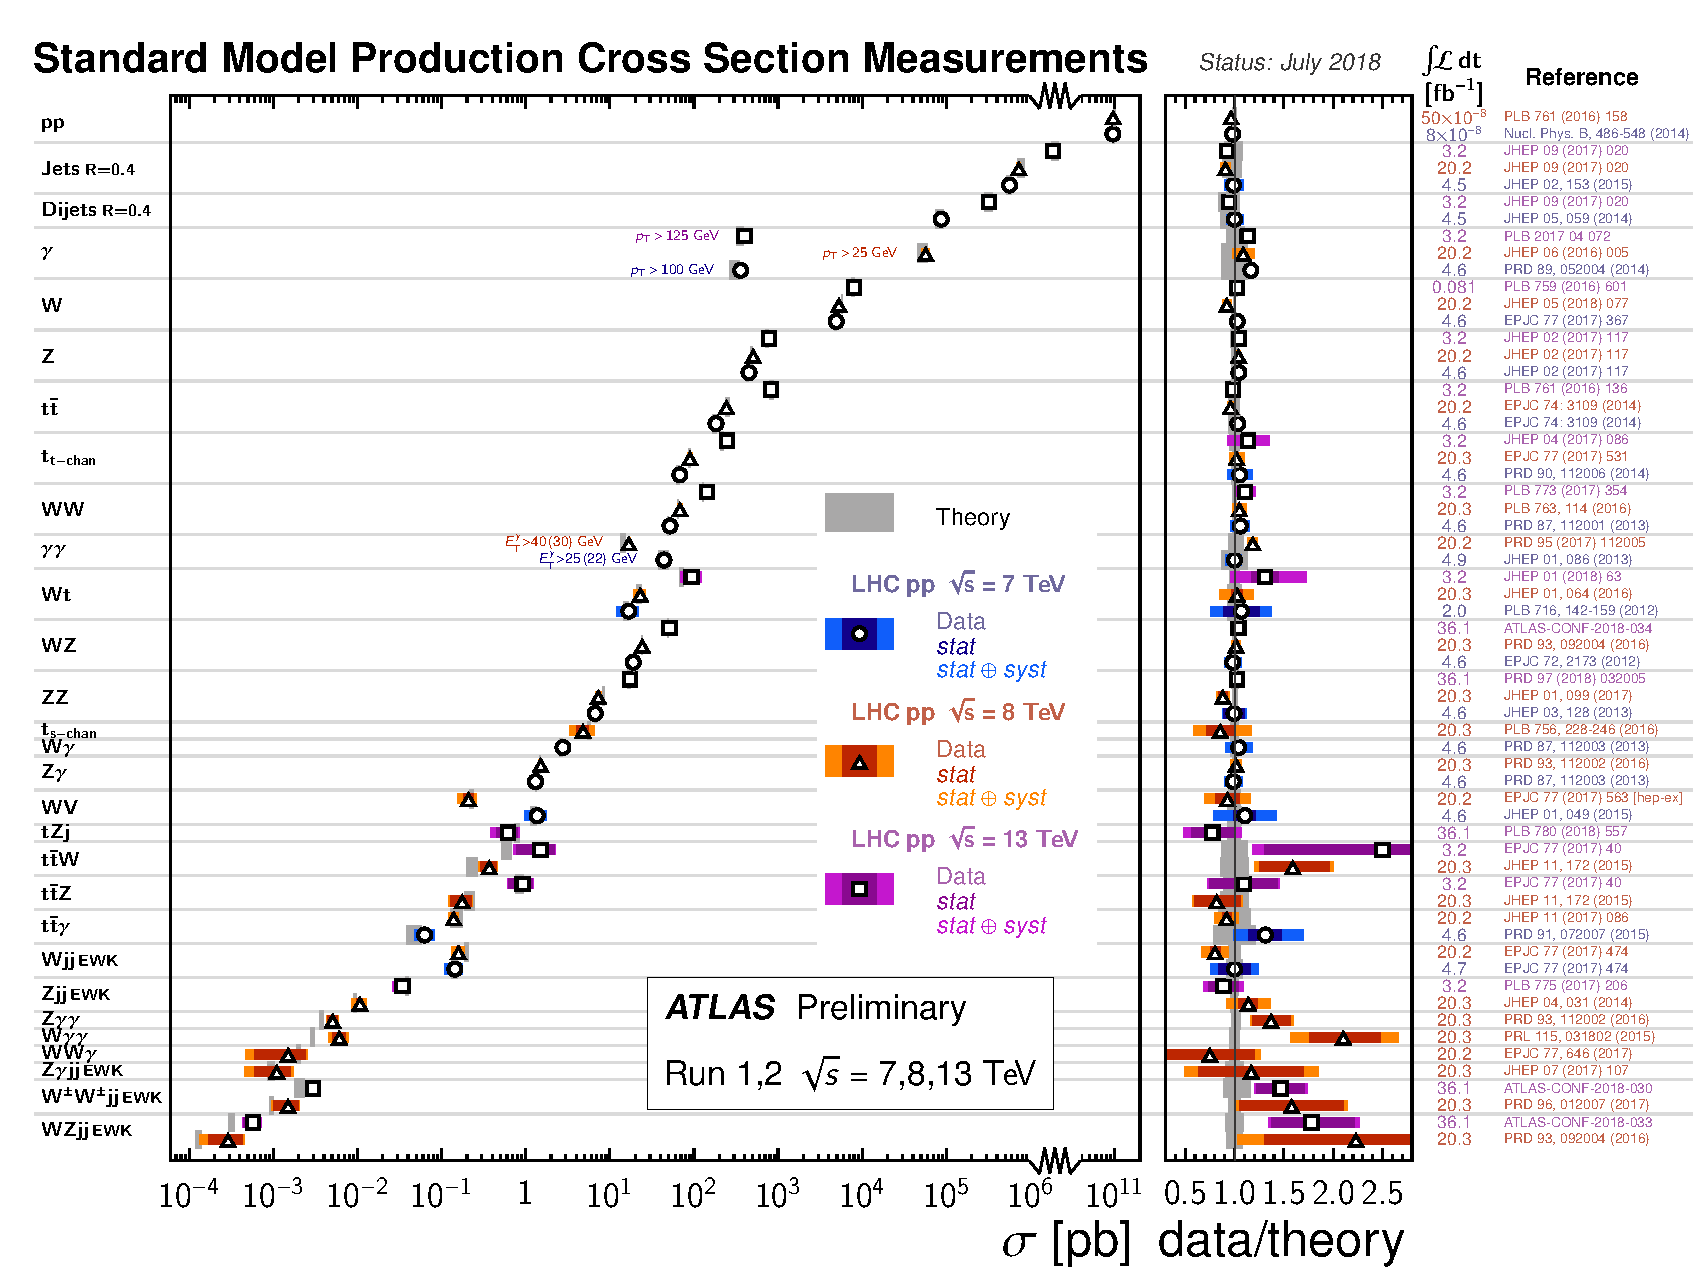
\includegraphics[width=\textwidth]{theory/ATLAS_SMSummary_FiducialXsect_rotated.eps}
 \caption[Summary of several Standard Model total and fiducial production cross section measurements using LHC proton-proton collisions, corrected for leptonic branching fractions, compared to the corresponding theoretical expectations.]{%
  Summary of several Standard Model total and fiducial production cross section measurements using LHC proton-proton collisions, corrected for leptonic branching fractions, compared to the corresponding theoretical expectations.
  All theoretical expectations were calculated at NLO or higher.
  The dark-color uncertainty bar represents the statistical uncertainty.
  The lighter-color uncertainty bar represents the full uncertainty, including systematics and luminosity uncertainties.
  The data/theory ratio, luminosity used and reference for each measurement are also shown.
  Uncertainties for the theoretical predictions are quoted from the original ATLAS papers.
  They were not always evaluated using the same prescriptions for PDFs and scales.
  The $W\gamma$ and $Z\gamma$ theoretical cross-sections have non-perturbative corrections applied to the NNLO fixed order calculations~\cite{STDM-2011-17}.
  Not all measurements are yet statistically significant~\cite{web:ATLAS_SM_summary_plots}.}
 \label{fig:cross_section_experiment_theory}
\end{figure}

The quanta of the quantum fields of the Standard Model are the particles of matter and the mediators of the fundamental forces of Nature, shown in \Cref{fig:Standard_Model}.
The spin-$1/2$ fermion fields result in the three ``generations'' of the six quarks and six leptons, which compose all matter in the Universe.
The leptons are divided into the electrically charged leptons --- the electron $(e)$, muon $(\mu)$, and tau $(\tau)$ --- and their electrically neutral neutrino counterparts --- ``flavor'' eigenstates of $\nu_{e}$, $\nu_{\mu}$, and $\nu_{\tau}$.
The quarks have fractional electric charge, with the up $(u)$, charm $(c)$, and top $(t)$ quarks having $+2/3$ elementary charge, and the down $(d)$, strange $(s)$, and bottom $(b)$ quarks having $-1/3$, as well as all of them carrying a ``color'' charge that allows them to participate in strong nuclear interactions.
They do not exist as free particles by themselves, but always in bound configurations of either two or three quarks, respectively known as ``mesons'' and ``baryons'' (e.g., pions and protons, respectively).
In addition to the matter particles are the five vector gauge bosons that are mediators of fundamental forces of Nature.
The photon $(\gamma)$ is the mediator of the electromagnetic force and interacts with all particles that carry electrical charge (i.e. the quarks, charged leptons, and charged vector bosons).
The weak nuclear force that governs nuclear interactions, such as beta decay, is mediated by the $W^{+}$, $W^{-}$, and $Z$ massive weak vector bosons.
The electrically charged $W$ bosons mediate charged flavor changing interactions between the quarks and the leptons (e.g., $c \to d + W^{+}$ and $e^{-} \to \bar{\nu}_{e} + W^{-}$), and the $Z$ boson mediates electrically neutral flavor changing interactions (e.g., $e^{+}e^{-} \to Z \to \mu^{+}\mu^{-}$ and charged lepton scattering from neutrinos).
The eight%
\footnote{As a result of the $\mathrm{SU}(3)$ symmetry.}
massless gluons mediate the strong nuclear force and so have couplings with all particles that have color charge: the quarks and the gluons themselves.
The coupling strength of the gluons varies with distance between color charged particles --- being extremely strong at close ranges and then sharply dropping of at the distance of confinement (approximately the radius of the proton).
Finally, the Higgs boson imparts mass to particles that it couples to, with stronger coupling strengths manifesting as larger masses.
This process --- which has been come to be known as the ``Higgs mechanism'' --- gives rise to the non-zero mass of the $W^{\pm}$ and $Z$ through a processes called ``electroweak symmetry breaking'' and will be discussed more throughly in \Cref{section:EWSB}.

\begin{figure}
 \centering
 \includegraphics[width=\textwidth]{theory/Standard_Model.pdf}
 \caption[Diagram of the particles of the Standard Model.]{%
  Diagram of the particles of the Standard Model.
  Shown are the three generations of fermions (the quarks and leptons), the gauge vector bosons (gluons, photon, $W^{\pm}$, and $Z$), and the Higgs boson.
  This figure was inspired and adapted from~\cite{web:Carsten_Burgard}.}
 \label{fig:Standard_Model}
\end{figure}

The following discussion of the theories that compose the Standard Model is my summary of many post-lecture conversations with former SMU professor Kent Hornbostel and readings of~\cite{Pich:2005mk}.

\section{Quantum Field Theories}\label{section:QFT}

\acrlong{QFT} is the mathematical framework for modern particle physics calculations.
QFT naturally incorporates quantum theory with special relativity to give a relativistic description of the interaction of quantum fields through their quantized excitations (particles).
All possible physical interactions of these fields are encoded in the terms of the Lagrangian density, $\Lagrangian$, which is a scalar and so (crucially) Lorentz invariant --- physics fundamentally works the same regardless of reference frame.
Given the ubiquity of the use of the Lagrangian density in calculations it will be interchangeably referred to as the ``Lagrangian'' henceforth, with hopefully minimal confusion.
Additionally, the Lagrangian density must be locally gauge invariant; meaning that it is invariant under certain Lie group transformations.
Local gauge invariance is an expression that representations of the Lagrangian density that result in the same physical interactions must be equivalently valid.
A local gauge symmetry is distinct from a global gauge symmetry, as would arise in Noether's theorem, in that a local gauge symmetry results in a gauge invariance for the spacetime point of consideration, but is not guaranteed to be valid in all cases.
That is, a global gauge symmetry is in some sense a special case of a local gauge symmetry, where the symmetry applies for all points.
As an example, consider the Dirac Lagrangian
\begin{equation}
 \Lagrangian_{\textrm{Dirac}} = \bar{\psi} \left(i \gamma^{\mu}\partial_{\mu} - m\right)\psi.
 \label{eq:Dirac_Lagrangian}
\end{equation}
If a global gauge transformation of a phase shift is applied,
\[
 \psi \to e^{-i\theta} \psi, \qquad \bar{\psi} \to \bar{\psi}\,e^{i\theta},
\]
then it is readily seen that the Lagrangian has remained invariant
\[
 \Lagrangian \to \bar{\psi} \left(i \gamma^{\mu}\partial_{\mu} - m\right)\psi.
\]
However, if a local gauge transformation of a phase shift dependent on the field's spacetime is applied
\[
 \psi \to e^{-i\theta(x)} \psi, \qquad \bar{\psi} \to \bar{\psi}\,e^{i\theta(x)},
\]
then for the Lagrangian
\[
 \Lagrangian \to \bar{\psi} \left(i \gamma^{\mu}\partial_{\mu} - m\right)\psi + \bar{\psi}\, \gamma^{\mu} \left(\partial_{\mu} \theta\right)\psi
\]
to preserve the definition of the four-gradient under such a local transformation requires the addition of a gauge field $A_{\mu}(x)$ to form the covariant%
\footnote{``Covariant'' in that it transforms with the gauge fields so that the derivative remains unchanged.}
derivative,
\[
 D_{\mu} \equiv \partial_{\mu} - iq A_{\mu}(x),
\]
with local gauge transformation
\[
 A_{\mu} \to A_{\mu} - \frac{1}{q} \partial_{\mu}\theta,
\]
such that
\[
 \theta(x) = q \Lambda(x),
\]
resulting in the nice covariant form
\[
 \Lagrangian \to \bar{\psi} \left(i \gamma^{\mu}D_{\mu} - m\right)\psi = \bar{\psi} \left(i \slashed{D} - m\right)\psi.
\]
Given the implications of local gauge invariance, the gauge may be arbitrarily chosen to simplify calculations with no less of generality.

Two examples of highly successful \glspl{QFT} are \gls{QED} and \gls{QCD}, which are briefly discussed here.

\subsection{Quantum Electrodynamics (QED)}\label{subsection:QED}

The Glashow-Weinberg-Salam theory of electromagnetic interactions~\cite{Glashow:1961tr,Goldstone:1962es,Weinberg:1967tq} defines electromagnetic interactions of matter in the Standard Model.
The Lagrangian density for QED --- which describes the interactions of a spin-$1/2$ field with the electromagnetic field --- possesses a global $\mathrm{U}(1)$ symmetry, manifest through the conservation of electric charge, and is given by
\begin{equation}
 \Lagrangian_{\textrm{QED}} = -\frac{1}{4}F_{\mu\nu} F^{\mu\nu} + \bar{\psi} \left(i \slashed{D} - m\right)\psi
 \label{eq:QED_Lagrangian}
\end{equation}
where $F_{\mu\nu} = \partial_{\mu}A_{\nu} - \partial_{\nu}A_{\mu}$ is the electromagnetic field strength tensor.
In the QED Lagrangian, the kinetic term $-\frac{1}{4}F_{\mu\nu} F^{\mu\nu}$ describes the behavior of the electromagnetic field --- which along with the Euler-Lagrange equations result in Maxwell's equations --- and the term $\bar{\psi} \left(i \slashed{D} - m\right)\psi$ gives the interactions of the electromagnetic field with charged particles.

\subsection{Quantum Chromodynamics (QCD)}\label{subsection:QCD}

\gls{QCD} is the gauge field theory that describes the interactions of quarks and gluons governed by the strong nuclear force, and characterized by a $\mathrm{SU}(3)$ symmetry.
The QCD Lagrangian density is
\begin{equation}
 \Lagrangian_{\textrm{QCD}} = -\frac{1}{4}G_{\mu \nu}^{a} G_{a}^{\mu \nu} + \sum_{f} i \bar{\psi}_{f} D_{\mu} \gamma^{\mu} \psi_{f},
 \label{eq:QCD_Lagrangian}
\end{equation}
for the $f$ families of quarks, $\psi_{f}$.
The Lagrangian is written without the color index for readability, but, as both the quarks and gluons carry a color charge, then the quark fields $\psi$ are column vectors with color index $\alpha$ and the gluon fields $G_{\mu}^{a}$ are matrices with color indices $\alpha$ and $\beta$.
The kinetic term $-\frac{1}{4}G_{\mu \nu}^{a} G_{a}^{\mu \nu}$ describes the self interactions of the gluon fields $G_{\mu}^{a}$ given the gluon field strength tensor $G_{\mu\nu}^{a} = \partial_{\mu} G_{\nu}^{a} - g_{s} f^{abc} G_{\mu}^{b} G_{\nu}^{c}$
for strong coupling constant $g_{s}$ and $\mathrm{SU}(3)$ structure constants $f^{abc}$.
The term $\sum_{f} i \bar{\psi}_{f} D_{\mu} \gamma^{\mu} \psi_{f}$ with covariant derivative
\[
 D_{\mu} = \partial_{\mu} - i g_{s} G_{\mu}^{a} T^{a},
\]
where $T^{a}$ are the generators of the $\mathrm{SU}(3)$ symmetry group, is the kinetic term for the quarks and describes the interactions between quarks and gluons.
All terms in the Lagrangian density that involve quarks and gluons are color singlets, which promotes the idea of ``color confinement.''
In Nature this color confinement is seen empirically by the observation of quarks only in bound states with other quarks that are colorless --- i.e., free quarks have never been directly observed.
These bound states of quarks are known as ``hadrons.''
Half-integer spin hadrons formed from an even number of quarks are known as ``mesons'', and integer spin hadrons formed from an odd number of quarks are known as ``baryons.''
In strong interactions at hadron colliders there is enough energy to break individual quarks and gluons out of their hadronic forms, however these free partons then immediately ``hadronize'' by forming bound states with other quarks, even if that requires sacrificing some of their energy to pull another quark from the vacuum.
This process of hadronization, and subsequent decays, creates a shower of hadrons and leptons that is collectively referred to as a ``jet'' and will be discussed more in \Cref{section:jets}.
Jets play an important role in understanding the physics of QCD, and the observation of three jet systems is the best experimental evidence of the existence of gluons~\cite{Brandelik:1979bd,Ellis:1978wp,Andersson:1983ia,Brandelik:1980vs}.

QCD is a deeply rich theory that deserves much attention (c.f.~\cite{Campbell:2017hsr}), but for the purposes of this thesis it will only be introduced here to motivate a more complete picture of the QFTs that build the Standard Model.

\section{Spontaneous Symmetry Breaking}\label{section:symmetry_breaking}

Spontaneous symmetry breaking is the process by which a physical system that has a symmetry does not express that symmetry for perturbations around the ground state of the system.
It is worth noting, given the somewhat confusing nature of the use of ``breaking,'' that the symmetry of the Lagrangian is not destroyed under symmetry breaking, but rather is not manifest given the ground state into which the system has been perturbed.
A classical example of spontaneous symmetry breaking is that of a pen being balanced upright on its tip on a table.
In the unstable equilibrium state of the pen being balanced (the high energy/excited state configuration) the pen possesses a $\mathrm{U}(1)$ symmetry of rotation about its axis.
If the pen is perturbed from this state by a small vibration it will fall into its ground state onto the surface of the table and will lie along some direction ``breaking'' the symmetry that was exhibited by the previous state.
Another example is that of Heisenberg’s model of the ferromagnet, which has Hamiltonian of $\mathcal{H} = -\sum_{i\neq j} J_{ij}\,\vec{s}_{i} \cdot \vec{s}_{j}$ across neighboring atoms.
This Hamiltonian also possesses as rotational symmetry above the Curie temperature --- rotating all the spins by some amount leaves the total spin of the system invariant.
However, below the Curie temperature a non-zero magnetization will arise along a particular direction which will cause all spins to become aligned parallel to it, breaking the symmetry.

A final illustrative toy model, that will prove useful in the context of the Higgs mechanism, is that of a massive complex scalar field
\[
 \phi = \frac{1}{\sqrt{2}} \left(\phi_{1} + i \phi_{2}\right),
\]
with Lagrangian density
\[
 \Lagrangian = \partial_{\mu}\phi^{\dagger}\partial^{\mu}\phi - m^{2}\phi^{\dagger}\phi + \frac{\lambda}{4} \left(\phi^{\dagger}\phi\right)^{2}
\]
composed of the kinetic term, $\partial_{\mu}\phi^{\dagger}\partial^{\mu}\phi$, and the potential $V\left(\phi\right) = -m^{2}\phi^{\dagger}\phi + \frac{\lambda}{4} \left(\phi^{\dagger}\phi\right)^{2}$.
The potential is zero at $\phi=0$, but has its minima occur at
\[
 \phi^{\dagger}\phi = \frac{1}{2}\left(\phi_{1}^{2} - \phi_{2}^{2}\right) = \frac{2m^2}{\lambda} \equiv \frac{1}{2}v^{2}
\]
with magnitude
\[
 \abs{\phi} = \frac{1}{\sqrt{2}}v = \frac{\sqrt{2} v}{\lambda^{1/2}}.
\]
It is seen that this potential possesses a $\mathrm{U}(1)$ symmetry, such that it is invariant under $\phi \to e^{-i\theta}\phi$, resulting in an infinite number of possible minima.
Rewriting the fields using polar coordinates in field space,
\[
 \phi(x) = \frac{1}{\sqrt{2}} \rho\left(x\right) e^{-i \theta(x)/v},
\]
and choosing the arbitrary ground state --- breaking the symmetry --- of $\rho=v$ and $\theta=0$ then allows for the redefinition of the fields as
\[
 \phi(x) = \frac{1}{\sqrt{2}} \left(v + h\left(x\right)\right) e^{-i \theta(x)/v},
\]
where $h$ and $\theta$ become the normal modes.
Perturbations about the minima result in massive radial $h$ modes and massless rotational $\theta$ modes.
These radial modes result in a massive particle, and the rotational modes result in massless particles known as Nambu-Goldstone bosons~\cite{Nambu:1960tm,Goldstone:1961eq}.

\section{Electroweak Symmetry and Interactions}\label{section:EW_interactions}

The electroweak interactions are encoded in the symmetry group $\mathrm{SU}(2)_{L} \otimes \mathrm{U}(1)_{Y}$, where $\mathrm{SU}(2)$ is the symmetry of weak-isospin and $Y$ is weak-hypercharge.
The gauge group requires all left-handed spinors to be doublets, and the right-handed spinors to be singlets.
Considering only the first generation of quarks and leptons, this can be written for the leptons as
\[
 \psi_{e\,1}\left(x\right) = \begin{pmatrix}
  \nu_{e} \\
  e^{-}
 \end{pmatrix}_{L},\quad
 \psi_{e\,2}\left(x\right) = \nu_{e\,R},\quad
 \psi_{e\,3}\left(x\right) = e_{R}^{-}\,,
\]
and for the quarks as
\[
 \psi_{u\,1}\left(x\right) = \begin{pmatrix}
  u \\
  d
 \end{pmatrix}_{L},\quad
 \psi_{u\,2}\left(x\right) = u_{R},\quad
 \psi_{u\,3}\left(x\right) = d_{R}\,.
\]
The ``free'' Lagrangian density (the kinetic term) is then
\[
 \Lagrangian = \sum_{j=1}^{3} i \,\bar{\psi}_{e\,j}\left(x\right) \slashed{\partial} \,\psi_{e\,j}\left(x\right) + i \,\bar{\psi}_{u\,j}\left(x\right) \slashed{\partial} \,\psi_{u\,j}\left(x\right)\,,
\]
which should be invariant under local gauge transformations of the symmetry group,
\[
 \begin{split}
  \psi_{e\,1}&\left(x\right) \to e^{iy_{1} \beta(x)}\, U_{L}\left(x\right)\psi_{e\,1}\left(x\right), \qquad U_{L}\left(x\right) = \exp\left(i\,\frac{\tau^{i}}{2} \alpha^{i}(x)\right)\\
  \psi_{e\,2}&\left(x\right) \to e^{iy_{2} \beta(x)}\, \psi_{e\,2}\left(x\right)\\
  \psi_{e\,3}&\left(x\right) \to e^{iy_{3} \beta(x)}\, \psi_{e\,3}\left(x\right)
 \end{split}
\]
The generators of $\mathrm{SU}(2)$ are the Pauli spin matrices,
\[
 \tau^{0} = \begin{pmatrix}%
  1 & 0 \\%
  0 & 1
 \end{pmatrix},\quad
 \tau^{1} = \begin{pmatrix}%
  0 & 1 \\%
  1 & 0
 \end{pmatrix},\quad
 \tau^{2} = \begin{pmatrix}%
  0 & -i \\%
  i & 0
 \end{pmatrix},\quad
 \tau^{3} = \begin{pmatrix}%
  1 & 0  \\%
  0 & -1 %
 \end{pmatrix}\,,%
\]
and the resulting four degrees of freedom (three from $\mathrm{SU}(2)$ and one from $\mathrm{U}(1)$) manifest as the gauge bosons of the weak vector fields $W_{\mu}^{k}\left(x\right)$:
\[
 B_{\mu}\left(x\right) = W_{\mu}^{0}\left(x\right)\tau^{0}, \qquad \vec{W}_{\mu}\left(x\right) = W_{\mu}^{i}\left(x\right)\frac{\tau^{i}}{2}\,.
\]
As a result, the covariant derivative is
\begin{align}
 D_{\mu}\psi_{1}(x) & = \left(\partial_{\mu} - ig_{1}\, y_{1} B_{\mu}(x) - ig_{2} \vec{W}_{\mu}(x)\right)\psi_{1}(x)\label{eq:EW_derivative} \\
 D_{\mu}\psi_{2}(x) & = \left(\partial_{\mu} - ig_{1}\, y_{2} B_{\mu}(x)\right)\psi_{2}(x)\notag                                             \\
 D_{\mu}\psi_{3}(x) & = \left(\partial_{\mu} - ig_{1}\, y_{3} B_{\mu}(x)\right)\psi_{3}(x)\notag
\end{align}
for weak hypercharge $y_{i}$ coupling $g_{1}$ and weak isospin coupling $g_{2}$, this gives the requirements for the local transformations of the vector gauge fields,
\[
 B_{\mu}(x) \to B_{\mu}(x) + \frac{1}{g_{1}} \partial_{\mu}\beta(x), \qquad%
 \vec{W}_{\mu}(x) \to U_{L}(x)\vec{W}_{\mu}(x)\,U_{L}^{\dagger}(x) - \frac{i}{g_{2}} \left(\partial_{\mu}U_{L}(x)\right)
 U_{L}^{\dagger}(x)
\]
The kinetic term of the electroweak vector gauge field Lagrangian density is then seen to be
\[
 \Lagrangian_{\textrm{kinetic}} = -\frac{1}{4}B_{\mu\nu}B^{\mu\nu} - \frac{1}{2}\mathrm{Tr}\left(\vec{W}_{\mu\nu}\vec{W}^{\mu\nu}\right) = -\frac{1}{4}B_{\mu\nu}B^{\mu\nu} -\frac{1}{4} W_{\mu\nu}^{i} W_{i}^{\mu\nu}.
\]
It is seen that the $\mathrm{SU}(2)_{L} \otimes \mathrm{U}(1)_{Y}$ gauge symmetry forbids a mass term for the vector fields, and fermion masses are also forbidden as the term would mix the left and right handed fields which have different transformation properties --- which would explicitly break the gauge symmetry.

\subsection{Electroweak Interactions}

Given the covariant derivative, \Cref{eq:EW_derivative}, and resulting Lagrangian density for the fermions,
\[
 \Lagrangian = \sum_{j=1}^{3} i \,\bar{\psi}_{e\,j}\left(x\right) \slashed{D} \,\psi_{e\,j}\left(x\right) + i \,\bar{\psi}_{u\,j}\left(x\right) \slashed{D} \,\psi_{u\,j}\left(x\right)\,,
\]
it is seen that there are interactions between the fermions and the vector gauge fields (dropping fermion index for compactness),
\[
 \Lagrangian \subset g_{2} \bar{\psi}_{1} \gamma^{\mu}\vec{W}_{\mu} \psi_{1} + g_{1} B_{\mu} \sum_{j=1}^{3} y_{j}\bar{\psi}_{j} \gamma^{\mu} \,\psi_{j}\,.
\]
The first term, which contains the $\mathrm{SU}(2)_{L}$ matrix
\[
 \vec{W}_{\mu} = W_{\mu}^{i}(x) \frac{\tau^{i}}{2} = \frac{1}{\sqrt{2}} \begin{pmatrix}%
  \sqrt{2} W_{\mu}^{3} & W_{\mu}^{\dagger}     \\
  W_{\mu}              & -\sqrt{2} W_{\mu}^{3}
 \end{pmatrix}\,,
\]
gives rise to the charged current interactions of the charged $W$ boson fields
\[
 W_{\mu} = \frac{1}{\sqrt{2}} \left(W_{\mu}^{1}  + i W_{\mu}^{2}\right), \qquad W_{\mu}^{\dagger} = \frac{1}{\sqrt{2}} \left(W_{\mu}^{1}  - i W_{\mu}^{2}\right)
\]
with the left-handed quarks and charged leptons, seen in \Cref{fig:EW_W_quarks} and \Cref{fig:EW_W_leptons}.
Likewise, through mixing of the neutral $W_{\mu}^{3}$ and $B_{\mu}$ fields,
\[
 \begin{pmatrix}
  A_{\mu} \\
  Z_{\mu}
 \end{pmatrix}
 = \begin{pmatrix}
  \cos\theta_{W}  & \sin\theta_{W} \\
  -\sin\theta_{W} & \cos\theta_{W}
 \end{pmatrix}
 \begin{pmatrix}
  B_{\mu} \\
  W_{\mu}^{3}
 \end{pmatrix}\,,
\]
with Weinberg mixing angle
\[
 \sin\theta_{W} = \frac{g_{1}}{\sqrt{g_{1}^{2} + g_{2}^{2}}}, \qquad \cos\theta_{W} = \frac{g_{2}}{\sqrt{g_{1}^{2} + g_{2}^{2}}},
\]
the mass eigenstates of the $Z$ boson and photon arise
\[
 \begin{split}
  Z_{\mu} &= W_{\mu}^{3} \cos\theta_{W} - B_{\mu} \sin\theta_{W} = \frac{1}{\sqrt{g_{1}^{2} + g_{2}^{2}}} \left(g_{2} W_{\mu}^{3} - g_{1} B_{\mu}\right) \\
  A_{\mu} &= W_{\mu}^3 \sin\theta_{W} + B_{\mu} \cos\theta_{W} = \frac{1}{\sqrt{g_{1}^{2} + g_{2}^{2}}} \left(g_{1} W_{\mu}^{3} + g_{2} B_{\mu}\right)
 \end{split}
\]
which mediate the neutral current interactions with the fermions, seen in \Cref{fig:EW_Z} and \Cref{fig:QED_photon}.

\begin{figure}[htbp]
 \centering
 \begin{subfigure}[t]{0.23\textwidth}
  \centering
  \includegraphics[width=\textwidth]{theory/QED_photon.pdf}
  \caption[The vertex for interactions of an electrically charged particle and a photon.]{%
   The vertex for interactions of an electrically charged particle and a photon.}
  \label{fig:QED_photon}
 \end{subfigure}%
 \quad
 \begin{subfigure}[t]{0.23\textwidth}
  \centering
  \includegraphics[width=\textwidth]{theory/electroweak_Z.pdf}
  \caption[The vertex for neutral current interactions of an fermion and a $Z$ boson.]{%
   The vertex for neutral current interactions of an fermion and a $Z$ boson.}
  \label{fig:EW_Z}
 \end{subfigure}%
 \quad
 \begin{subfigure}[t]{0.23\textwidth}
  \centering
  \includegraphics[width=\textwidth]{theory/electroweak_W_quarks.pdf}
  \caption[The vertex for charged current interactions of quarks with a $W$ boson.]{%
   The vertex for charged current interactions of quarks with a $W$ boson.}
  \label{fig:EW_W_quarks}
 \end{subfigure}%
 \quad
 \begin{subfigure}[t]{0.23\textwidth}
  \centering
  \includegraphics[width=\textwidth]{theory/electroweak_W_leptons.pdf}
  \caption[The vertex for charged current interactions of a charged lepton and neutrino with a $W$ boson.]{%
   The vertex for charged current interactions of a charged lepton and neutrino with a $W$ boson.}
  \label{fig:EW_W_leptons}
 \end{subfigure}%
 \caption[The Feynman diagrams for allowed QED and electroweak interactions.]{%
  The Feynman diagrams for allowed QED and electroweak interactions in the Standard Model.}
 \label{fig:electroweak_vertices}
\end{figure}

\section{Electroweak Symmetry Breaking}\label{section:EWSB}

To break the electroweak symmetry and provide masses to the weak vector bosons, consider the discussion given in \Cref{section:symmetry_breaking} and a complex scalar doublet (introduced by, among others~\cite{Guralnik:1964eu,Kibble:2015mwa}, Brout and Englert~\cite{Englert:1964et}, and Higgs~\cite{Higgs:1964ia,Higgs:1964pj})
\begin{equation}
 \phi = \begin{pmatrix}%
  \phi^{+} \\%
  \phi^{0}
 \end{pmatrix} = \frac{1}{\sqrt{2}} \begin{pmatrix}%
  \phi_{1} + i \phi_{2} \\%
  \phi_{3} + i \phi_{4}%
 \end{pmatrix}%
 \label{eq:Higgs_doublet}
\end{equation}
with Lagrangian density
\begin{equation}
 \Lagrangian_{\textrm{Higgs}} = \left(D_{\mu}\phi\right)^{\dagger}D^{\mu}\phi - \mu^{2}\phi^{\dagger}\phi + \lambda \left(\phi^{\dagger}\phi\right)^{2}
 \label{eq:Higgs_Lagrangian}
\end{equation}
that is invariant under local $\mathrm{SU}(2)_{L} \otimes \mathrm{U}(1)_{Y}$ transformations.
The Higgs potential
\begin{equation}
 V\left(\phi\right) = -\mu^{2}\phi^{\dagger}\phi + \lambda \left(\phi^{\dagger}\phi\right)^{2},
 \label{eq:Higgs_potential}
\end{equation}
shown in \Cref{fig:Higgs_potential}, is chosen such that $\mu^{2} < 0$ and $\lambda > 0$ to provide stable minima.
As before in \Cref{section:symmetry_breaking} with the case of the toy model of the massive complex scalar field, once a ground state has been arbitrarily chosen this spontaneously breaks the $\mathrm{SU}(2)_{L} \otimes \mathrm{U}(1)_{Y}$ symmetry to the subgroup $\mathrm{U}(1)_{\textrm{QED}}$.
This time, the four fields of the complex scalar doublet are reparameterized into
\[
 \phi(x) = \frac{1}{\sqrt{2}} \begin{pmatrix}
  0 \\
  v + h(x)
 \end{pmatrix}
 \exp\left(i \frac{\tau^{i}}{2} \theta^{i}(x)\right)
\]
which gives the real scalar field $h(x)$, corresponding to radial perturbations of the minima, and three%
\footnote{There is much beauty in electroweak symmetry breaking, but the simple, insightful choice of the doublet to give as many Nambu-Goldstone bosons as vector gauge fields is marvelous.}
Nambu-Goldstone fields $\theta^{i}(x)$ with rotational symmetry --- their values have become gauge choices.
Exploiting this gauge freedom, and choosing the unitary gauge $\theta^{i}(x)=0$, results in kinetic term $\left(\textrm{where } g = \sqrt{g_{1}^{2} + g_{2}^{2}}\right)$
\[
 \Lagrangian \subset \frac{1}{2}\partial_{\mu} h \partial^{\mu} h + \left(v + h\right)^{2} \left(\frac{g^{2}}{4} W_{\mu}^{\dagger}W^{\mu} + \frac{g^{2}}{8 \cos^2 \theta_{W}} Z_{\mu}^{\dagger}Z^{\mu}\right)
\]
where the $W^{\pm}$ and $Z$ bosons have absorbed the Nambu-Goldstone bosons as polarizations and respectively acquired masses of
\[
 m_{W} = \frac{1}{2}vg, \qquad m_{Z} = \frac{m_{W}}{\cos\theta_{W}} = \frac{vg}{2\cos\theta_{W}}\,.
\]
The scalar field --- the Higgs field --- also acquires a mass term of
\[
 m_{h} = \sqrt{-2\mu^{2}} = \sqrt{2h}v.
\]
In the Standard Model $v$, $g_{1}$, $g_{2}$ are free parameters to be measured by experiment, and so the masses of the bosons are not directly predicted.
However, the value%
\footnote{Often referred to as the ``weak scale'' or the ``vacuum expectation value.''}
of $v$ has been calculated independently~\cite{Plehn:2005nk} to be approximately $246~\GeV$.
It is also noted that in further interactions the quarks and charged leptons acquire a mass term from Yukawa couplings~\cite{Yukawa:1935xg}, $c_i$, with the Higgs field
\[
 \begin{split}
  \Lagrangian_{\textrm{Yukawa}} &= -\frac{1}{\sqrt{2}} \left(v+h\right) \left(c_{1}\bar{d}d + c_{2}\bar{u}u + c_{3}\bar{e}e\right) \\
  &= - \left(1 + \frac{h}{v}\right)\left(m_{d}\bar{d}d + m_{u}\bar{u}u + m_{e}\bar{e}e\right)\,.
 \end{split}
\]
The neutrinos notably do not participate in this interaction, and their observed non-zero mass~\cite{Ahmad:2001an} is unexplained through electroweak symmetry breaking in the Standard Model and is currently unresolved.

\begin{figure}[htbp]
 \centering
 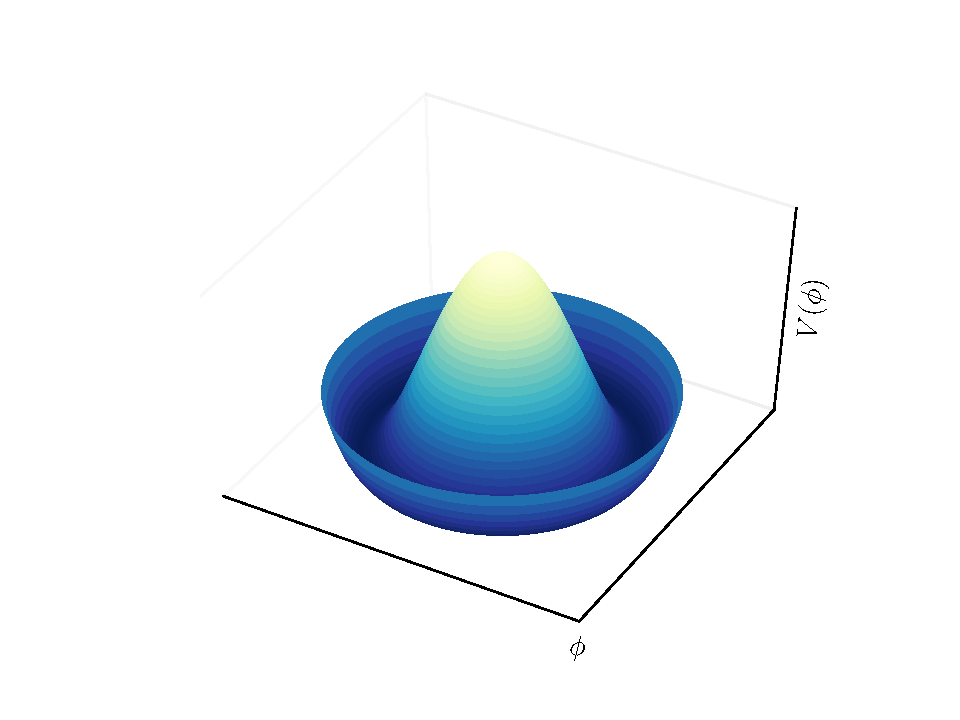
\includegraphics[width=\linewidth]{theory/higgs_potential.pdf}
 \caption[Sketch of the Higgs potential shape.]{%
 Sketch of the Higgs potential's ``wine bottle'' shape.
 The trough (the bottom of the eponymous wine bottle) are the infinite choices of minima at the vacuum expectation value, $v$, that can be selected upon spontaneously breaking the $\mathrm{SU}(2)_{L} \otimes \mathrm{U}(1)_{Y}$ symmetry to the subgroup $\mathrm{U}(1)_{\textrm{QED}}$.}
 \label{fig:Higgs_potential}
\end{figure}

\section{The Higgs Boson}\label{section:Higgs_boson}

The massive Higgs boson produced though the ``Higgs mechanism'' approach to electroweak symmetry breaking is a particle of great interest, as the interactions of the Higgs field with all other elementary particle fields generates their mass.
As a result, through these couplings the Higgs boson can be produced through a large number of interactions.
As this thesis is focused on experimental efforts at CERN's \gls{LHC}, the production mechanisms of interest will be the leading ones in a hadron collider with center-of-mass energy $\sqrt{s}=13~\TeV$.
In order of decreasing cross section, those production modes are: gluon-gluon fusion (ggF), vector boson fusion (VBF), vector boson-associated production or ``Higgsstrahlung'' (VH), and associated production with $t\bar{t}$ ($t\bar{t}H$) and $b\bar{b}$ ($b\bar{b}H$), seen in \Cref{fig:Higgs_production_diagrams}.
The predicted cross section for these production modes are given in \Cref{table:Higgs_production_cross_section} and plotted with theory uncertainties in \Cref{fig:Higgs_production_cross_section_theory}.

\begin{figure}[htbp]
 \centering
 \begin{subfigure}[t]{0.48\textwidth}
  \centering
  \includegraphics[width=\textwidth]{theory/Higgs_ggF.pdf}
  \caption[Feynman diagram for Higgs production through gluon-gluon fusion.]{%
   Feynman diagram for Higgs production through gluon-gluon fusion.}
  \label{fig:Higgs_ggF}
 \end{subfigure}%
 \quad
 \begin{subfigure}[t]{0.48\textwidth}
  \centering
  \includegraphics[width=\textwidth]{theory/Higgs_VBF.pdf}
  \caption[Feynman diagram for Higgs production through vector boson fusion.]{%
   Feynman diagram for Higgs production through vector boson fusion.}
  \label{fig:Higgs_VBF}
 \end{subfigure}%

 \begin{subfigure}[t]{0.48\textwidth}
  \centering
  \includegraphics[width=\textwidth]{theory/Higgs_strahlung.pdf}
  \caption[Feynman diagram for Higgs production through vector boson associated production (Higgsstrahlung).]{%
   Feynman diagram for Higgs production through vector boson associated production (Higgsstrahlung).}
  \label{fig:Higgs_associated_production}
 \end{subfigure}%
 \quad
 \begin{subfigure}[t]{0.48\textwidth}
  \centering
  \includegraphics[width=\textwidth]{theory/Higgs_ttbar_associated.pdf}
  \caption[Feynman diagram for Higgs production through associated production with heavy quarks ($t\bar{t}$ and $b\bar{b}$).]{%
   Feynman diagram for Higgs production through associated production with with heavy quarks ($t\bar{t}$ and $b\bar{b}$).}
  \label{fig:Higgs_associated_production_ttbar}
 \end{subfigure}%
 \caption[The leading production modes at the LHC for Higgs bosons.]{%
  The leading production modes at the LHC for Higgs bosons.}
 \label{fig:Higgs_production_diagrams}
\end{figure}

\begin{table}[htpb]
 \centering
 \caption[The Standard Model Higgs boson production cross sections in units of pb for $m_{H}=125~\GeV$ in $pp$ collisions as a function of the center-of-mass energy, $\sqrt{s}$, at the LHC.]{%
  The SM Higgs boson production cross sections in units of pb for $m_{H}=125~\GeV$ in $pp$ collisions as a function of the center-of-mass energy, $\sqrt{s}$, at the LHC.
  The predictions for the ggF channel include the latest N3LO results leading to reduced theoretical uncertainties by a factor around 2 compared to the N2LO results~\cite{PDG2018:Ch11,deFlorian:2016spz}.}
 \begin{tabular}{@{}rrrrrrrr@{}} \toprule
  $\sqrt{s}~(\TeV)$ & ggF                  & VBF                  & $WH$                 & $ZH$                 & $t\bar{t}H$           & $b\bar{b}H$            & Total~(pb) \\ \midrule
  $13$              & $48.6_{-5\%}^{+5\%}$ & $3.78_{-2\%}^{+2\%}$ & $1.37_{-2\%}^{+2\%}$ & $0.88_{-5\%}^{+5\%}$ & $0.50_{-13\%}^{+9\%}$ & $0.49_{-24\%}^{+20\%}$ & $55.59$    \\
  \addlinespace[0.3em]
  $14$              & $54.7_{-5\%}^{+5\%}$ & $4.28_{-2\%}^{+2\%}$ & $1.51_{-2\%}^{+2\%}$ & $0.99_{-5\%}^{+5\%}$ & $0.60_{-13\%}^{+9\%}$ & $0.55_{-24\%}^{+20\%}$ & $62.65$    \\
  \bottomrule
 \end{tabular}\label{table:Higgs_production_cross_section}%
\end{table}

\begin{figure}
 \centering
 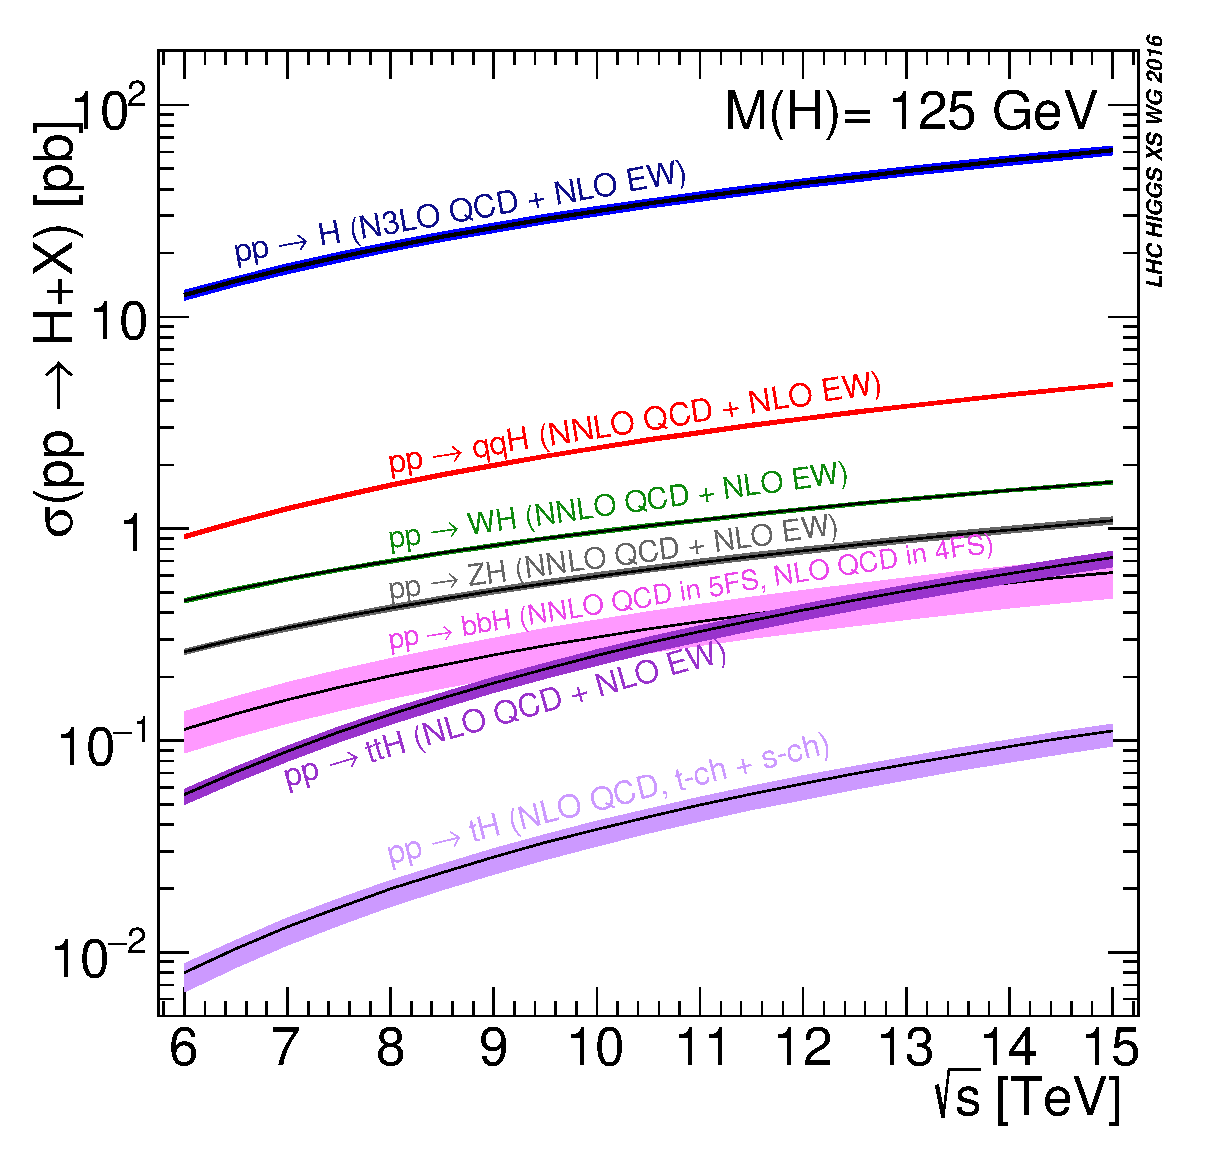
\includegraphics[width=0.5\textwidth]{theory/Higgs_XS_7-14TeV-2016.eps}
 \caption[The Standard Model Higgs boson production cross sections as a function of the center-of-mass energy, $\sqrt{s}$, for $pp$ collisions.]{%
  The Standard Model Higgs boson production cross sections as a function of the center-of-mass energy, $\sqrt{s}$, for $pp$ collisions.
  The VBF process is indicated as $qqH$.
  The theoretical uncertainties are indicated as bands~\cite{PDG2018:Ch11}.}
 \label{fig:Higgs_production_cross_section_theory}
\end{figure}

The SM Higgs has couplings to all the massive vector gauge fields and charged fermions, and so can decay into all of their particles.
At leading order the Higgs will decay primarily to a pair of $b$-quarks $(b\bar{b})$, a pair of weak vector bosons with one of them being off-shell $(VV^{*})$, a pair of gluons $(gg)$, a pair of tau leptons $(\tau^{+}\tau^{-})$, or a pair of photons $(\gamma\gamma)$.
The decays to massless gauge bosons (gluons and photons) are facilitated through loops of massive particles.
The Feynman diagrams for these decays are shown in \Cref{fig:Higgs_decay_channels}, listed in descending (observed) branching ratio in \Cref{table:Higgs_BRs}, and plotted with theory uncertainties in \Cref{fig:Higgs_BRs}.
As the Higgs Yukawa couplings are proportional to the mass of the decay products, it is seen that the Higgs primarily decays to $b\bar{b}$ as $m_{H} < 2 m_{t}$.
However, as hadron colliders mostly produce multijet events%
\footnote{Discovery machines are a messy business.}
from QCD processes, identifying jets coming from resonant $H \to b\bar{b}$ events is quite challenging.

\begin{figure}[htbp]
 \centering
 \begin{subfigure}[t]{0.48\textwidth}
  \centering
  \includegraphics[width=\textwidth]{theory/Hbb.pdf}
  \caption[Feynman diagram for Higgs decay to $b\bar{b}$.]{%
   Feynman diagram for Higgs decay to $b\bar{b}$.}
  \label{fig:H_to_bb}
 \end{subfigure}
 \quad
 \begin{subfigure}[t]{0.48\textwidth}
  \centering
  \includegraphics[width=\textwidth]{theory/H_WW.pdf}
  \caption[Feynman diagram for Higgs decay to $WW^{*}$.]{%
   Feynman diagram for Higgs decay to $WW^{*}$.}
  \label{fig:H_to_WW}
 \end{subfigure}

 \begin{subfigure}[t]{0.48\textwidth}
  \centering
  \includegraphics[width=\textwidth]{theory/Hgg.pdf}
  \caption[Feynman diagram for Higgs decay to $gg$.]{%
   Feynman diagram for Higgs decay to $gg$.}
  \label{fig:H_to_gg}
 \end{subfigure}
 \quad
 \begin{subfigure}[t]{0.48\textwidth}
  \centering
  \includegraphics[width=\textwidth]{theory/Htautau.pdf}
  \caption[Feynman diagram for Higgs decay to $\tau^{+}\tau^{-}$.]{%
   Feynman diagram for Higgs decay to $\tau^{+}\tau^{-}$.}
  \label{fig:H_to_tautau}
 \end{subfigure}

 \begin{subfigure}[t]{0.48\textwidth}
  \centering
  \includegraphics[width=\textwidth]{theory/H_ZZ.pdf}
  \caption[Feynman diagram for Higgs decay to $ZZ^{*}$.]{%
   Feynman diagram for Higgs decay to $ZZ^{*}$.}
  \label{fig:H_to_ZZ}
 \end{subfigure}
 \quad
 \begin{subfigure}[t]{0.48\textwidth}
  \centering
  \includegraphics[width=\textwidth]{theory/H_photons.pdf}
  \caption[Feynman diagram for Higgs decay to $\gamma\gamma$.]{%
   Feynman diagram for Higgs decay to $\gamma\gamma$.}
  \label{fig:H_to_photons}
 \end{subfigure}
 \caption[The leading decay channels of the Higgs boson.]{%
  The leading decay channels of the Higgs boson.}
 \label{fig:Higgs_decay_channels}
\end{figure}

\begin{table}[htpb]
 \centering
 \caption[The branching ratios and the relative uncertainty for a Standard Model Higgs boson with $m_{H}=125~\GeV$.]^{+3.2\%}$ \\
  \addlinespace[0.3em]
  $H\to W^{+}W^{-}$       & $2.14 \times 10^{-1}$ & $_{-4.2\%}^{+4.3\%}$ \\
  \addlinespace[0.3em]
  $H\to \tau^{+}\tau^{-}$ & $6.27 \times 10^{-2}$ & $_{-5.7\%}^{+5.7\%}$ \\
  \addlinespace[0.3em]
  $H\to ZZ$               & $2.62 \times 10^{-2}$ & $_{-4.1\%}^{+4.3\%}$ \\
  \addlinespace[0.3em]
  $H\to \gamma\gamma$     & $2.27 \times 10^{-3}$ & $_{-4.9\%}^{+5.0\%}$ \\
  \addlinespace[0.3em]
  $H\to Z\gamma$          & $1.53 \times 10^{-3}$ & $_{-8.9\%}^{+9.0\%}$ \\
  \addlinespace[0.3em]
  $H\to \mu^{+}\mu^{-}$   & $2.18 \times 10^{-4}$ & $_{-5.9\%}^{+6.0\%}$ \\
  \bottomrule
 \end{tabular}\label{table:Higgs_BRs}%
\end{table}

\begin{figure}
 \centering
 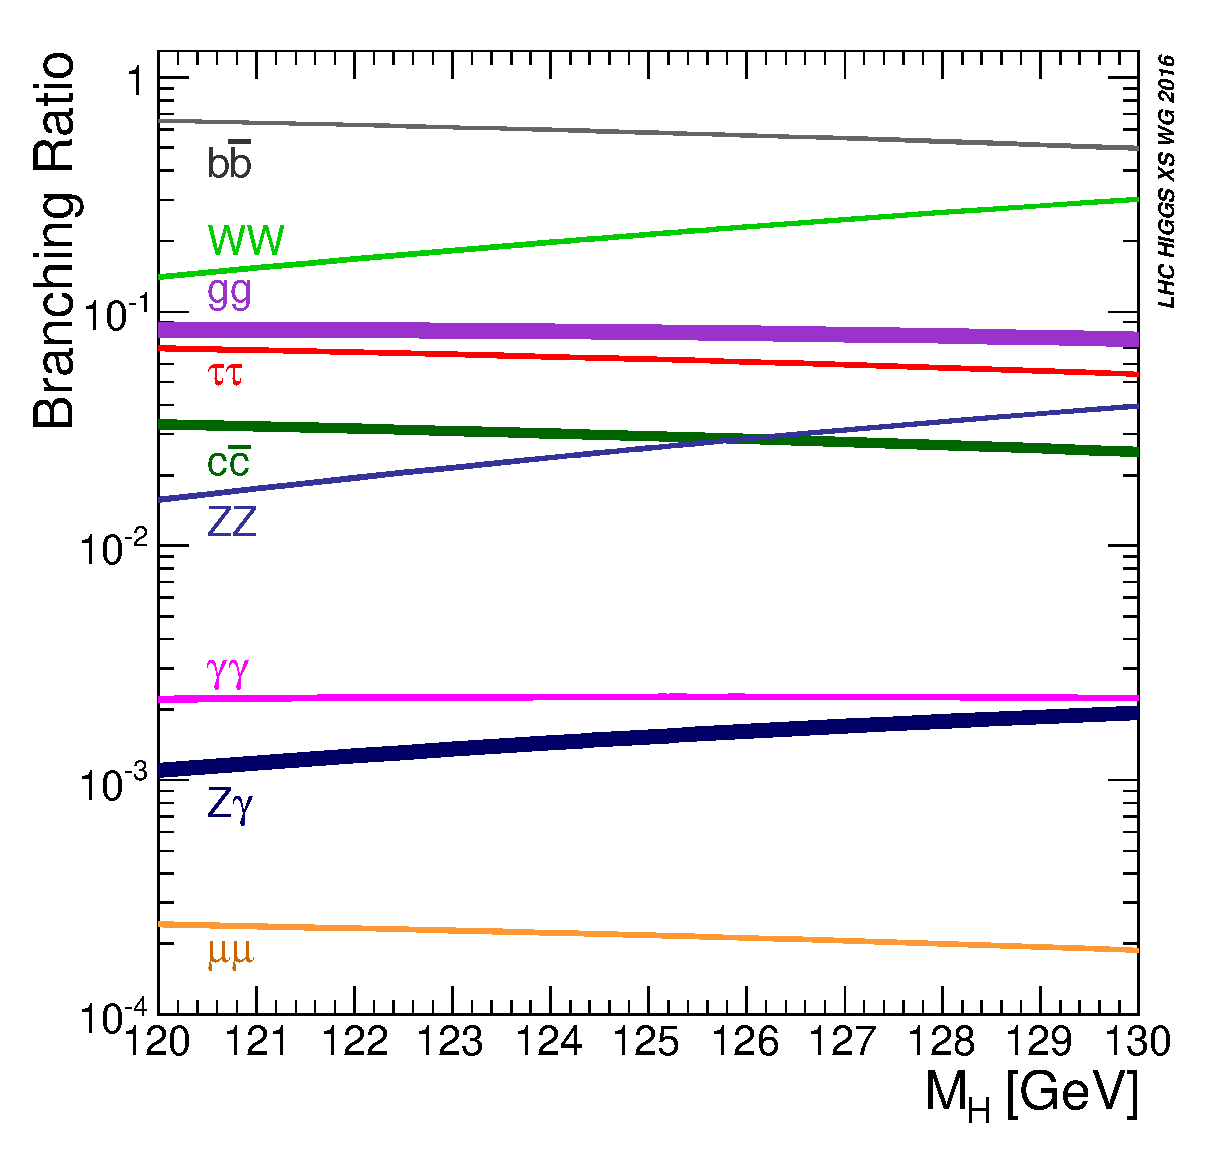
\includegraphics[width=0.5\textwidth]{theory/SMHiggsBR.eps}
 \caption[The branching ratios for the main decays of the Standard Model Higgs boson near $m_{H}=125~\GeV$.]{%
  The branching ratios for the main decays of the Standard Model Higgs boson near $m_{H}=125~\GeV$.
  The theoretical uncertainties are indicated as bands~\cite{PDG2018:Ch11}.}
 \label{fig:Higgs_BRs}
\end{figure}

\section{Extensions to the Standard Model}

From astronomical observations of the rotation speeds of galaxies~\cite{Rubin:1970zza,Begeman:1991iy}, precision measurements of the cosmic microwave background~\cite{2013ApJS:darkmatter,Akrami:2018vks}, and gravitational lensing measurements~\cite{Trimble:10.1146,Bertone:2004pz,Feng:2010gw}, there is evidence that in addition to the normal matter of the Standard Model in the Universe there exists ``dark matter'' that constitutes approximately $26.8\%$ of the energy density of the Universe.
Dark matter is so far seen to interact with normal matter only through gravitation.
As it does not interact with normal matter through the electroweak or strong nuclear force, any interactions with normal matter are outside of the Standard Model.

To incorporate a model of particle dark matter there are a number of existing extensions of the Standard Model.
Among these are frameworks of simplified dark matter models~\cite{EXOT-2017-32,Jacques:2016dqz,Kahlhoefer:2015bea,Alves:2015pea} where new particles mediate the interactions of dark matter, $\chi$, with the Standard Model particles.
Among these are models for a single neutral vector mediator particle: a $\Zprime$.
One simple extension of the standard model is a vector or axial-vector simplified model through an additional $\mathrm{U}(1)$ gauge symmetry which gives dark matter particles a charge of this symmetry group~\cite{Abercrombie:2015wmb}, and results in either a vector $\left(Z'_{V}\right)$ or axial-vector $\left(Z'_{A}\right)$ boson mediator.
This model introduces five new parameters: the mass of the mediator, $m_{\Zprime}$, the mass of the Dirac fermion dark matter particle, $m_{\chi}$, the flavor-universal coupling of the $\Zprime$ to SM quarks, $g_{q}$, the coupling of the $\Zprime$ to all lepton flavors, $g_{\ell}$, and the coupling of the $\Zprime$ to dark matter, $g_{\chi}$.
The resulting interactions of the $\Zprime$ mediator and the particles are shown in \Cref{fig:Zprime_interactions}.

\begin{figure}[htbp]
 \centering
 \begin{subfigure}[t]{0.48\textwidth}
  \centering
  \includegraphics[width=\textwidth]{theory/Zprime_SM_coupling.pdf}
  \caption[Feynman diagram of the interactions of the $\Zprime$ mediator with Standard Model fermions.]{%
   Feynman diagram of the interactions of the $\Zprime$ mediator with Standard Model fermions.}
  \label{fig:Zprime_SM_coupling}
 \end{subfigure}%
 \quad
 \begin{subfigure}[t]{0.48\textwidth}
  \centering
  \includegraphics[width=\textwidth]{theory/Zprime_DM_coupling.pdf}
  \caption[Feynman diagram of the interactions of the $\Zprime$ mediator with dark matter.]{%
   Feynman diagram of the interactions of the $\Zprime$ mediator with dark matter.}
  \label{fig:Zprime_DM_coupling}
 \end{subfigure}%
 \caption[Feynman diagrams of the interactions of the $\Zprime$ mediator with both Standard Model fermions and dark matter.]{%
  Feynman diagrams of the interactions of the $\Zprime$ mediator with both Standard Model fermions and dark matter.}
 \label{fig:Zprime_interactions}
\end{figure}

For the purposes of the analysis done in this thesis only fully hadronic final states are of interest, and so a leptophobic $\left(g_{\ell}=0\right)$ $\Zprime$ model is considered.
This model then introduces the additional term to the Lagrangian density for a vector model of
\[
 \Lagrangian_{\textrm{vector}} = g_{q} \sum_{q} Z^{\prime}_{\mu} \bar{q} \gamma^{\mu} q + g_{\chi} Z^{\prime}_{\mu} \bar{\chi} \gamma^{\mu} \chi
\]
and for an axial-vector model
\[
 \Lagrangian_{\textrm{axial-vector}} = g_{q} \sum_{q} Z^{\prime}_{\mu} \bar{q} \gamma^{\mu}\gamma^{5} q + g_{\chi} Z^{\prime}_{\mu} \bar{\chi} \gamma^{\mu}\gamma^{5} \chi
\]
where $q$ and $\chi$ are respectively the Dirac spinors for the SM quark and dark matter fields and $g_{q}$ is democratic with respect to all quark flavors.
